\documentclass[11pt,a4paper]{article}

\usepackage[T1]{fontenc}
\usepackage[utf8]{inputenc}
\usepackage[spanish,es-nodecimaldot]{babel}
\usepackage{lmodern}
\usepackage{geometry}
\usepackage{amsmath,amssymb}
\usepackage{booktabs,longtable,tabularx,array}
\usepackage{graphicx}
\usepackage{pdflscape}
\usepackage{xcolor}
\usepackage{siunitx}
\usepackage{enumitem}
\usepackage{microtype}
\usepackage{fancyhdr}
\usepackage{hyperref}

\geometry{top=20mm,bottom=22mm,left=20mm,right=20mm}
\setlength{\parindent}{0pt}
\setlength{\parskip}{5pt}
\setlength{\headheight}{14pt}
\setlist[itemize]{leftmargin=5mm,itemsep=2pt,topsep=3pt}
\setlist[enumerate]{leftmargin=6mm,itemsep=2pt,topsep=3pt}
\makeatletter
\renewcommand{\numberline}[1]{\hb@xt@3em{#1\hfil}}
\makeatother

\definecolor{pampablue}{HTML}{174A6E}
\definecolor{pampagreen}{HTML}{2E6B57}
\definecolor{pampaorange}{HTML}{B56820}
\definecolor{lightblue}{HTML}{EAF2F7}
\definecolor{lightorange}{HTML}{FFF3E5}
\definecolor{lightgreen}{HTML}{EAF5F0}

\hypersetup{
  colorlinks=true,
  linkcolor=pampablue,
  urlcolor=pampablue,
  citecolor=pampagreen,
  pdftitle={Memoria de calculo del front-end ARINC 429-like con TL082CP},
  pdfauthor={Proyecto PAMPA}
}

\sisetup{
  output-decimal-marker={,},
  per-mode=symbol,
  range-phrase={ a },
  range-units=single
}
\DeclareSIUnit{\bit}{bit}
\DeclareSIUnit{\baud}{Bd}

\pagestyle{fancy}
\fancyhf{}
\lhead{Proyecto PAMPA}
\rhead{Memoria de cálculo del front-end}
\cfoot{\thepage}
\renewcommand{\headrulewidth}{0.4pt}

\newcommand{\importantbox}[2]{%
  \begin{center}
  \fcolorbox{#1}{#1!7}{\parbox{0.92\textwidth}{\textbf{#2}}}
  \end{center}
}

\newcommand{\component}[1]{\texttt{#1}}

\begin{document}

\begin{titlepage}
  \centering
  \vspace*{18mm}
  {\Large\color{pampablue}\textbf{PROYECTO PAMPA}\par}
  \vspace{12mm}
  {\Huge\bfseries Memoria de cálculo\par}
  \vspace{4mm}
  {\LARGE Front-end eléctrico ARINC 429-like\par}
  \vspace{3mm}
  {\Large TL082CP + MCP6562\par}
  \vspace{14mm}

  \fcolorbox{pampablue}{lightblue}{%
    \parbox{0.82\textwidth}{
      \centering
      Justificación de ganancias, impedancias, referencias, desacople,
      adaptación de línea y respuesta temporal para
      \SI{100}{\kilo\bit\per\second} y
      \SI{12.5}{\kilo\bit\per\second}.
    }
  }

  \vfill
  {\large Documento asociado al esquemático\par}
  \vspace{2mm}
  {\ttfamily frontend\_arinc429\_tl082\_circuit.kicad\_sch\par}
  \vspace{10mm}
  {\large \today\par}
\end{titlepage}

\tableofcontents
\newpage

\section{Alcance y criterio de diseño}

Esta memoria justifica los valores del circuito vigente mediante las ecuaciones
de los amplificadores diferenciales, las cargas vistas por las Raspberry Pi
Pico, la impedancia característica de la línea y la respuesta temporal de los
dispositivos. El objetivo es construir un banco que reproduzca los niveles y
la temporización principales de ARINC 429 para un transmisor y un receptor.

Los valores eléctricos de referencia se toman del tutorial ARINC 429 provisto
con el proyecto. Los parámetros del TL082CP se toman de la hoja de datos de
Texas Instruments aportada al proyecto. Para el MCP6562 se usa su hoja de datos
oficial de Microchip.

\importantbox{pampaorange}{La adaptación ARINC no consiste en colocar
\SI{78}{\ohm} en el receptor. La fuente se aproxima a
\SI{75}{\ohm} balanceados y el receptor debe ser de alta impedancia. Por ello
puede existir una reflexión inicial en el extremo receptor; lo que se busca es
que la fuente absorba el retorno y que los flancos controlados eviten reflexiones
repetidas, sobreimpulso y ringing.}

\subsection{Objetivos de referencia}

\begin{table}[h]
\centering
\caption{Magnitudes eléctricas y temporales usadas como objetivo.}
\begin{tabularx}{\textwidth}{@{}>{\bfseries}l X l@{}}
\toprule
Magnitud & Objetivo & Uso en el cálculo \\
\midrule
Cable & Par trenzado blindado, $Z_0\approx\SI{78}{\ohm}$ & Adaptación de fuente \\
Impedancia TX & $\SI{75}{\ohm}\pm\SI{5}{\ohm}$, repartida entre A y B & $R_9+R_{10}$ \\
Impedancia RX & $Z_{in}\geq\SI{8}{\kilo\ohm}$ & Redes de \SI{100}{\kilo\ohm} \\
Niveles TX & $+\SI{10}{V}$, $0$ y $-\SI{10}{V}$ diferenciales & Ganancia TX $1{,}5$ \\
100 kbps & $T_b=\SI{10}{\micro\second}$, media celda \SI{5}{\micro\second} & Verificación rápida \\
12,5 kbps & $T_b=\SI{80}{\micro\second}$, media celda \SI{40}{\micro\second} & Verificación lenta \\
Flanco rápido & $\SI{1.5}{\micro\second}\pm\SI{0.5}{\micro\second}$ & Conformado opcional \\
Flanco lento & $\SI{10}{\micro\second}\pm\SI{5}{\micro\second}$ & Conformado opcional \\
\bottomrule
\end{tabularx}
\end{table}

\section{Etapa transmisora con U1 TL082CP}

\subsection{Elección de alimentación}

El TL082CP no es rail-to-rail. Su hoja de datos recomienda alimentaciones
simétricas entre $\pm\SI{5}{V}$ y $\pm\SI{15}{V}$ y, para la versión utilizada,
indica un rango de modo común aproximado desde $V_{CC-}+\SI{4}{V}$ hasta
$V_{CC+}-\SI{4}{V}$. Con $\pm\SI{12}{V}$ ese rango es aproximadamente
$-\SI{8}{V}$ a $+\SI{8}{V}$, suficiente para los nodos internos del circuito.

Cada conductor debe alcanzar aproximadamente $\pm\SI{4.95}{V}$. La alimentación
$\pm\SI{12}{V}$ deja margen respecto del swing de salida, mientras que
$\pm\SI{6}{V}$ quedaría demasiado cerca de los rieles. Por ello se adopta:

\[
  U1:\qquad V^+=+\SI{12}{V},\qquad V^-=-\SI{12}{V}.
\]

\subsection{Ganancia diferencial: R1--R8}

En U1A se usan $R_1=R_3=\SI{20}{\kilo\ohm}$ y
$R_2=R_4=\SI{30}{\kilo\ohm}$. La razón de resistencias es

\[
  k=\frac{R_2}{R_1}=\frac{R_4}{R_3}
   =\frac{\SI{30}{\kilo\ohm}}{\SI{20}{\kilo\ohm}}=1{,}5.
\]

Para un amplificador diferencial con razones apareadas:

\[
  V_{TXA\_DRV}=k\,(V_{TX\_A}-V_{TX\_B}).
\]

U1B repite el circuito con entradas intercambiadas:

\[
  V_{TXB\_DRV}=k\,(V_{TX\_B}-V_{TX\_A}).
\]

Con lógica de \SI{3.3}{V}:

\begin{align*}
  V_{TXA\_DRV} &= 1{,}5(3{,}3-0)=+\SI{4.95}{V},\\
  V_{TXB\_DRV} &= 1{,}5(0-3{,}3)=-\SI{4.95}{V},\\
  V_{AB} &= V_A-V_B\approx \SI{9.9}{V}.
\end{align*}

Al invertir las entradas se obtiene $V_{AB}\approx-\SI{9.9}{V}$; cuando ambas
entradas son iguales se obtiene el estado NULL, aproximadamente \SI{0}{V}
diferencial. Así, la relación $30/20$ convierte los \SI{3.3}{V} lógicos en los
tres estados buscados sin exigir que un GPIO entregue tensión negativa.

Los cuatro pares $R_1/R_2$, $R_3/R_4$, $R_5/R_6$ y $R_7/R_8$ deben conservar
la misma razón. Con resistencias independientes de \SI{1}{\percent}, el peor
caso de ganancia es

\[
  k_{max}=1{,}5\frac{1{,}01}{0{,}99}=1{,}5303,\qquad
  k_{min}=1{,}5\frac{0{,}99}{1{,}01}=1{,}4703.
\]

La salida diferencial nominal quedaría aproximadamente entre
\SI{9.70}{V} y \SI{10.10}{V}, todavía dentro del objetivo de
$\pm\SI{10}{V}\pm\SI{1}{V}$. Para mejorar rechazo de modo común y simetría se
recomiendan resistencias de \SI{1}{\percent} como mínimo; una red apareada de
\SI{0.1}{\percent} mejora la repetibilidad.

\subsection{Carga vista por los GPIO}

Cada GPIO alimenta un camino inversor de \SI{20}{\kilo\ohm} y un camino no
inversor de aproximadamente $\SI{20}{\kilo\ohm}+\SI{30}{\kilo\ohm}$.
Una estimación conservadora es

\[
 Z_{GPIO}\approx \SI{20}{\kilo\ohm}\parallel\SI{50}{\kilo\ohm}
 =\SI{14.29}{\kilo\ohm}.
\]

La corriente máxima aproximada suministrada por un GPIO alto es

\[
 I_{GPIO}\approx\frac{\SI{3.3}{V}}{\SI{14.29}{\kilo\ohm}}
 =\SI{0.231}{\milli\ampere}.
\]

Esta corriente es pequeña y explica por qué se eligieron decenas de
kiloohmios en lugar de resistencias de pocos cientos de ohmios. Aumentarlas
demasiado elevaría la sensibilidad a ruido, fugas y capacidad parásita; bajarlas
no aporta precisión y cargaría innecesariamente la Pico.

\subsection{Impedancia de salida: R9 y R10}

Se colocan $R_9=R_{10}=\SI{39}{\ohm}$, una por conductor. La impedancia
diferencial de fuente queda

\[
 Z_{out,diff}\approx R_9+R_{10}+2Z_{out,CL}
 \approx\SI{78}{\ohm},
\]

donde $Z_{out,CL}$ es la impedancia de salida en lazo cerrado del TL082. La
realimentación la reduce, pero no se dispone de un valor garantizado para toda
frecuencia; por eso no se afirma que sea exactamente cero. Las resistencias de
\SI{39}{\ohm} son las que dominan y hacen repetible la adaptación.

Con resistencias de \SI{1}{\percent}, la suma queda entre
\SI{77.22}{\ohm} y \SI{78.78}{\ohm}. Con \SI{5}{\percent} podría alcanzar
\SI{81.9}{\ohm}, por encima del máximo de \SI{80}{\ohm} asociado al objetivo
$\SI{75}{\ohm}\pm\SI{5}{\ohm}$; por eso aquí se recomienda \SI{1}{\percent}.

El coeficiente de reflexión visto en la fuente es

\[
 \Gamma_S=\frac{Z_S-Z_0}{Z_S+Z_0}.
\]

Para $Z_S=Z_0=\SI{78}{\ohm}$, $\Gamma_S=0$. Incluso tomando el nominal ARINC
de \SI{75}{\ohm} frente a un cable de \SI{78}{\ohm}, resulta
$\Gamma_S=-0{,}0196$, es decir, cerca de \SI{2}{\percent} en magnitud.

\subsection{Carga de uno y varios receptores}

Con el RX diseñado, $Z_{in,diff}\approx\SI{100}{\kilo\ohm}$, de modo que

\[
 V_{RX}\approx\SI{9.9}{V}
 \frac{\SI{100}{\kilo\ohm}}{\SI{100}{\kilo\ohm}+\SI{78}{\ohm}}
 =\SI{9.892}{V}.
\]

Incluso con el mínimo de \SI{8}{\kilo\ohm}, la tensión sería
\SI{9.804}{V}. Esto confirma que una carga RX alta conserva la amplitud.

En cambio, veinte receptores de exactamente \SI{8}{\kilo\ohm} equivalen a
\SI{400}{\ohm}; la corriente diferencial sería del orden de
\SI{20.7}{\milli\ampere} y la amplitud bajaría a \SI{8.28}{V}. El TL082CP no
es un line-driver ARINC dedicado y esa condición de veinte cargas no queda
garantizada por este banco. El dimensionamiento actual está orientado a un
receptor de laboratorio.

\section{Línea J2 y reflexiones}

J2 transporta \component{LINE\_A}, \component{LINE\_B} y una referencia de
banco. El medio objetivo es un par trenzado blindado de
$Z_0\approx\SI{78}{\ohm}$.

El receptor ARINC no termina la línea con \SI{78}{\ohm}; debe presentar al
menos \SI{8}{\kilo\ohm}. Por eso, para el RX de \SI{100}{\kilo\ohm}:

\[
 \Gamma_L=\frac{Z_L-Z_0}{Z_L+Z_0}
 =\frac{100000-78}{100000+78}=0{,}9984.
\]

Esta reflexión positiva en el extremo de alta impedancia es esperable. La
resistencia serie de la fuente hace que la onda reflejada sea absorbida al
regresar, mientras que el rise/fall controlado reduce sobreimpulso y ringing.
Por lo tanto, el objetivo técnico correcto no es ``cero reflexión en ambos
extremos'', sino fuente adaptada, receptor de alta impedancia, cable adecuado y
flancos suficientemente lentos.

En cables muy cortos, cuyo retardo de propagación es mucho menor que el tiempo
de subida, el conjunto se aproxima a un circuito concentrado. En longitudes de
campo la impedancia característica y el trazado del par pasan a ser críticos.

\section{Etapa receptora analógica con U2 TL082CP}

\subsection{Atenuación y desplazamiento: R11--R18}

El circuito vigente usa $R_{in}=\SI{100}{\kilo\ohm}$ y
$R_f=\SI{10}{\kilo\ohm}$, por lo que

\[
 a=\frac{R_f}{R_{in}}=0{,}1.
\]

Con razones apareadas y referencia $V_{REF}$, las dos salidas son

\begin{align*}
 V_{RXA\_BIASED} &= V_{REF}+0{,}1(V_A-V_B),\\
 V_{RXB\_BIASED} &= V_{REF}+0{,}1(V_B-V_A).
\end{align*}

La Sección~5.1 demuestra que el divisor vigente queda cargado por las dos redes
de entrada y entrega $V_{REF}\approx\SI{1.5125}{V}$, no
\SI{1.65}{V}. Con ese valor real y $V_{AB}=\pm\SI{9.9}{V}$:

\begin{center}
\begin{tabular}{@{}lcc@{}}
\toprule
Estado de línea & $V_{RXA\_BIASED}$ & $V_{RXB\_BIASED}$ \\
\midrule
$V_{AB}=+\SI{9.9}{V}$ & \SI{2.5025}{V} & \SI{0.5225}{V} \\
$V_{AB}=\SI{0}{V}$ & \SI{1.5125}{V} & \SI{1.5125}{V} \\
$V_{AB}=-\SI{9.9}{V}$ & \SI{0.5225}{V} & \SI{2.5025}{V} \\
\bottomrule
\end{tabular}
\end{center}

La atenuación $0{,}1$ mantiene incluso $\pm\SI{13}{V}$ diferenciales dentro del
dominio del comparador alimentado a \SI{3.3}{V}. En ese extremo:

\[
 \SI{0.2125}{V}\leq V_{RX\_BIASED}\leq\SI{2.8125}{V}.
\]

\subsection{Impedancia de entrada del receptor}

La resistencia intrínseca de entrada del TL082 es del orden de
$10^{12}\,\Omega$, por lo que la impedancia la fijan R11--R18. Para excitación
diferencial balanceada, $V_A=+V_d/2$, $V_B=-V_d/2$ y la referencia es masa en
pequeña señal. Sumando las corrientes de las dos ramas asociadas a un conductor
se obtiene, para la red apareada $\SI{100}{\kilo\ohm}/\SI{10}{\kilo\ohm}$,

\[
 I_A=\frac{V_d}{\SI{220}{\kilo\ohm}}
     +\frac{V_d}{\SI{183.33}{\kilo\ohm}}
     =\frac{V_d}{\SI{100}{\kilo\ohm}}.
\]

Por lo tanto:

\[
 Z_{in,diff}=\frac{V_d}{I_A}\approx\SI{100}{\kilo\ohm}.
\]

El valor supera por un factor de $12{,}5$ el mínimo de
\SI{8}{\kilo\ohm}. En modo común, cada conductor encuentra dos caminos de
aproximadamente \SI{110}{\kilo\ohm}, por lo que
$Z_{in,CM}\approx\SI{110}{\kilo\ohm}\parallel\SI{110}{\kilo\ohm}
=\SI{55}{\kilo\ohm}$.
La elección de \SI{100}{\kilo\ohm} reduce la carga sobre la línea sin recurrir
a valores tan grandes que vuelvan dominantes las fugas y capacidades parásitas.

\subsection{Impedancia de salida de U2}

R12 y R16 son resistencias de realimentación, no resistencias serie de salida.
La impedancia de salida de cada canal es la del TL082 reducida por la ganancia
de lazo. Como U2 sólo conduce una entrada de comparador de impedancia muy alta y
una pista local corta, no se necesita adaptación a \SI{78}{\ohm} después de U2.
El requisito de línea se aplica en J2, no entre U2 y U3.

U2 también se alimenta con $\pm\SI{12}{V}$. Aunque su salida útil está entre
aproximadamente \SI{0.35}{V} y \SI{2.95}{V}, la fuente bipolar mantiene al
TL082 dentro de su rango de modo común y evita usarlo fuera de especificación.

\section{Referencias y decisión digital}

\subsection{VREF: R21, R22 y C10}

R21 y R22 valen \SI{10}{\kilo\ohm}. Si el divisor estuviera descargado,
entregaría

\[
 V_{REF}=\SI{3.3}{V}
 \frac{\SI{10}{\kilo\ohm}}
 {\SI{10}{\kilo\ohm}+\SI{10}{\kilo\ohm}}
 =\SI{1.65}{V}.
\]

Sin embargo, R14 y R18 conectan VREF a LINE\_A y LINE\_B mediante un camino de
$\SI{10}{\kilo\ohm}+\SI{100}{\kilo\ohm}$ cada uno. Con modo común de línea
aproximadamente nulo, ambos caminos equivalen a una carga de
$\SI{110}{\kilo\ohm}\parallel\SI{110}{\kilo\ohm}=\SI{55}{\kilo\ohm}$ hacia
masa. El valor real se obtiene de

\[
 R_{B,eq}=\SI{10}{\kilo\ohm}\parallel\SI{55}{\kilo\ohm}
 =\SI{8.462}{\kilo\ohm},
\]

\[
 V_{REF,cargado}=\SI{3.3}{V}
 \frac{\SI{8.462}{\kilo\ohm}}
 {\SI{10}{\kilo\ohm}+\SI{8.462}{\kilo\ohm}}
 =\SI{1.5125}{V}.
\]

La corriente de polarización del TL082 es despreciable frente a la corriente
del divisor, pero la carga resistiva de R14/R18 no lo es. Ésta es una corrección
necesaria respecto del cálculo ideal.

Con C10=\SI{100}{\nano\farad}:

\[
 R_{TH,cargado}=\SI{10}{\kilo\ohm}\parallel\SI{10}{\kilo\ohm}
 \parallel\SI{55}{\kilo\ohm}=\SI{4.583}{\kilo\ohm},
\]

\[
 \tau_{REF}=R_{TH,cargado}C=\SI{458}{\micro\second},\qquad
 f_c=\frac{1}{2\pi R_{TH,cargado}C}=\SI{347}{Hz}.
\]

Este capacitor filtra la referencia; no está en serie con la señal ARINC y no
deforma los bits.

El par \SI{10}{\kilo\ohm}/\SI{10}{\kilo\ohm} funciona para los niveles
nominales del banco, pero no queda justificado como referencia exacta de
\SI{1.65}{V}. Antes del PCB se recomienda una de estas correcciones:

\begin{itemize}
  \item referencia bufferizada de \SI{1.65}{V}; o
  \item R21=\SI{1}{\kilo\ohm} y R22=\SI{1.02}{\kilo\ohm}, que con la carga de
  \SI{55}{\kilo\ohm} entregan aproximadamente \SI{1.651}{V}; o
  \item como cambio mínimo, mantener R21=\SI{10}{\kilo\ohm} y usar
  R22=\SI{12.2}{\kilo\ohm}, que compensa la carga nominal y entrega
  aproximadamente \SI{1.649}{V}.
\end{itemize}

\subsection{VTH: R23, R24 y C11}

Con R23=\SI{5.6}{\kilo\ohm} y R24=\SI{10}{\kilo\ohm}:

\[
 V_{TH}=\SI{3.3}{V}
 \frac{\SI{10}{\kilo\ohm}}
 {\SI{5.6}{\kilo\ohm}+\SI{10}{\kilo\ohm}}
 =\SI{2.115}{V}.
\]

Con el divisor vigente cargado, el nivel activo nominal es \SI{2.5025}{V} y
NULL es \SI{1.5125}{V}. Los márgenes reales son:

\[
 M_{activo}=2{,}5025-2{,}1154=\SI{0.387}{V},\qquad
 M_{NULL}=2{,}1154-1{,}5125=\SI{0.603}{V}.
\]

El umbral queda desplazado hacia el nivel activo. Su resistencia de Thévenin es
\SI{3.59}{\kilo\ohm}. Con C11=\SI{100}{\nano\farad} se obtiene
$\tau=\SI{359}{\micro\second}$ y $f_c=\SI{443}{Hz}$.

Para el mínimo nivel válido de recepción, $V_{AB}=\SI{6.5}{V}$, U2 sólo entrega
\SI{2.1625}{V} en el canal activo y el margen actual baja a apenas
\SI{47}{\milli\volt}. El valor de \SI{5.6}{\kilo\ohm} queda justificado sólo
para el banco nominal de $\pm\SI{10}{V}$.

Si primero se corrige VREF a \SI{1.65}{V}, un valor alternativo
R23=\SI{6.8}{\kilo\ohm} produce $V_{TH}=\SI{1.964}{V}$, con unos
\SI{314}{\milli\volt} respecto de NULL y \SI{336}{\milli\volt} respecto del
activo mínimo. Si se conserva VREF cargado en \SI{1.5125}{V}, el umbral
equilibrado sería aproximadamente \SI{1.838}{V}, que requiere
R23$\approx\SI{7.96}{\kilo\ohm}$ con R24=\SI{10}{\kilo\ohm}. La solución más
coherente es corregir VREF y luego adoptar R23=\SI{6.8}{\kilo\ohm}.

\subsection{U3 MCP6562 y C9}

U3 se alimenta con \SI{3.3}{V}. El MCP6562 admite \SIrange{1.8}{5.5}{V}, tiene
entrada rail-to-rail, salida push-pull compatible con CMOS/TTL, histéresis
interna y retardo máximo especificado de aproximadamente \SI{80}{ns} en las
condiciones de ensayo. La salida nunca adopta los rieles $\pm\SI{12}{V}$ del
TL082, por lo que constituye la frontera segura hacia los GPIO de la Pico RX.

En el esquemático vigente, la señal sesgada entra en la entrada inversora y
$V_{TH}$ en la no inversora. En consecuencia, la salida lógica es
\textbf{activa en bajo}. Si el firmware necesitara lógica activa en alto, deben
intercambiarse las entradas del comparador o invertir la interpretación por
software.

C9=\SI{100}{\nano\farad} es el desacople local de U3. Debe ubicarse físicamente
entre VDD y VSS, lo más cerca posible de sus pines.

\section{Capacitores de alimentación C1--C9}

U1A y U1B son dos canales dentro del mismo encapsulado U1; por eso comparten un
único par de pines de alimentación y un único conjunto de desacople. Lo mismo
ocurre con U2A/U2B. No falta un juego de capacitores para el amplificador
``inferior'': eléctricamente ambos canales usan los mismos rieles.

\begin{longtable}{@{}p{30mm}p{25mm}p{105mm}@{}}
\toprule
Componentes & Valor & Justificación \\
\midrule
\endhead
C1, C3 & \SI{100}{\nano\farad} & Desacople de alta frecuencia de los rieles $+\SI{12}{V}$ y $-\SI{12}{V}$ de U1. TI recomienda \SI{0.1}{\micro\farad} cerámico cerca de cada pin de alimentación. \\
C2, C4 & \SI{10}{\micro\farad} & Reserva local de energía de U1 frente a variaciones más lentas de corriente y a la impedancia de cables/fuente. \\
C5, C7 & \SI{100}{\nano\farad} & Desacople de alta frecuencia de los dos rieles de U2. \\
C6, C8 & \SI{10}{\micro\farad} & Reserva local de energía de U2. \\
C9 & \SI{100}{\nano\farad} & Desacople del MCP6562 entre \SI{3.3}{V} y GND. \\
\bottomrule
\end{longtable}

Como referencia ideal, la reactancia de \SI{100}{\nano\farad} es
\SI{15.9}{\ohm} a \SI{100}{kHz} y \SI{127}{\ohm} a \SI{12.5}{kHz}; la de
\SI{10}{\micro\farad} es \SI{0.159}{\ohm} y \SI{1.27}{\ohm}, respectivamente.
En la práctica, ESR, ESL y trazado importan, de ahí la combinación de un
cerámico pequeño y un capacitor bulk.

No se usan capacitores de acople en serie con A o B: eliminarían la componente
continua necesaria para representar el estado NULL y producirían droop y
desplazamiento de línea de base.

\section{Slew rate, ancho de banda y rise time}

\subsection{Límite propio del TL082CP}

La hoja de datos aportada indica $SR_{typ}=\SI{13}{V\per\micro\second}$ y un
valor mínimo de tabla de \SI{8}{V\per\micro\second} bajo sus condiciones de
ensayo. Cada conductor cambia aproximadamente \SI{4.95}{V} entre NULL y activo.
Como A y B se mueven simultáneamente en sentidos opuestos, el tiempo diferencial
es el mismo que el de cada canal, no el doble:

\begin{align*}
 t_{SR,typ}&=\frac{\SI{4.95}{V}}
 {\SI{13}{V\per\micro\second}}=\SI{0.381}{\micro\second},\\
 t_{SR,min}&=\frac{\SI{4.95}{V}}
 {\SI{8}{V\per\micro\second}}=\SI{0.619}{\micro\second}.
\end{align*}

El ancho de banda de ganancia unitaria típico es \SI{3}{MHz}. Para la etapa TX,
la ganancia de ruido aproximada es $1+R_f/R_{in}=2{,}5$, por lo que

\[
 f_{CL}\approx\frac{\SI{3}{MHz}}{2{,}5}=\SI{1.2}{MHz},\qquad
 t_{r,BW}\approx\frac{0{,}35}{f_{CL}}=\SI{0.292}{\micro\second}.
\]

El valor dominante es entonces el slew rate, y se espera un rise time sin
conformado del orden de \SIrange{0.38}{0.62}{\micro\second}, sujeto a carga,
capacitancias y dispersión real.

Para U2, la ganancia de ruido es aproximadamente $1+0{,}1=1{,}1$:

\[
 f_{CL,RX}\approx\SI{2.73}{MHz},\qquad
 t_{r,BW,RX}\approx\SI{0.128}{\micro\second}.
\]

El comparador suma como máximo unos \SI{80}{ns} de propagación bajo las
condiciones de su hoja de datos, por lo que el acondicionamiento RX es mucho más
rápido que una media celda de \SI{5}{\micro\second}.

\subsection{Comparación con las dos velocidades}

\begin{table}[h]
\centering
\caption{Relación entre rise time y temporización de bit.}
\begin{tabularx}{\textwidth}{@{}lrrrrX@{}}
\toprule
Modo & Bit & Media celda & $t_r$ objetivo & $t_{r,TL082}$ & Lectura \\
\midrule
100 kbps & \SI{10}{\micro\second} & \SI{5}{\micro\second} & \SIrange{1}{2}{\micro\second} & \SIrange{0.38}{0.62}{\micro\second} & El TL082 es suficientemente rápido, pero el flanco bruto es más rápido que ARINC. \\
12,5 kbps & \SI{80}{\micro\second} & \SI{40}{\micro\second} & \SIrange{5}{15}{\micro\second} & \SIrange{0.38}{0.62}{\micro\second} & La holgura temporal es enorme; se necesita más conformado si se busca la forma de onda de baja velocidad. \\
\bottomrule
\end{tabularx}
\end{table}

Tomando el peor valor de slew de \SI{0.619}{\micro\second}, un único flanco
ocupa aproximadamente \SI{12.4}{\percent} de la media celda rápida y
\SI{1.55}{\percent} de la lenta. El TL082 no hace perder una fracción crítica
del bit; el problema es el opuesto: el flanco puede ser demasiado abrupto y
generar más energía de alta frecuencia, sobreimpulso y ringing.

Como estimación conservadora de meseta, restando subida y bajada a la media
celda, el TL082 bruto deja al menos

\[
 \SI{5}{\micro\second}-2(\SI{0.619}{\micro\second})
 =\SI{3.762}{\micro\second}
\]

en alta velocidad y \SI{38.762}{\micro\second} en baja. Esta cuenta es una
aproximación geométrica, no una definición normativa de tiempo útil.

\subsection{Conformado de flancos recomendado}

Los capacitores C1--C11 del esquemático son de alimentación o referencia y no
controlan el rise time de A/B. Para aproximar la pendiente ARINC sin cargar la
salida con un capacitor grande sobre el cable, puede evaluarse una compensación
apareada en la realimentación de U1.

Si se coloca un capacitor C0G/NP0 en paralelo con cada resistencia de
\SI{30}{\kilo\ohm} de la etapa TX (R2, R4, R6 y R8), manteniendo los cuatro
valores apareados, la constante dominante aproximada es

\[
 \tau=R_fC_f,\qquad t_r\approx2{,}2R_fC_f.
\]

Para alta velocidad:

\[
 C_{f,100k}\approx
 \frac{\SI{1.5}{\micro\second}}
 {2{,}2\cdot\SI{30}{\kilo\ohm}}
 =\SI{22.7}{pF}.
\]

Se puede iniciar con \SI{22}{pF}, que da $t_r\approx\SI{1.45}{\micro\second}$.
Para baja velocidad:

\[
 C_{f,12k5}\approx
 \frac{\SI{10}{\micro\second}}
 {2{,}2\cdot\SI{30}{\kilo\ohm}}
 =\SI{151.5}{pF}.
\]

Un valor de \SI{150}{pF} da $t_r\approx\SI{9.9}{\micro\second}$.

No debe usarse un único valor para ambos modos si se pretende cumplir las dos
ventanas de rise/fall. La solución práctica es una red conmutable
\SI{22}{pF}/\SI{150}{pF}, o un transmisor ARINC dedicado. Antes de incorporarla
al PCB deben simularse estabilidad y respuesta transitoria y luego verificarse
en osciloscopio. Los cuatro capacitores deben ser iguales para no degradar la
simetría y el rechazo de modo común.

Un capacitor diferencial grande directamente entre A y B no es la primera
opción con TL082: un escalón de \SI{10}{V} a través de \SI{78}{\ohm} puede
exigir una corriente transitoria inicial de aproximadamente
$\SI{10}{V}/\SI{78}{\ohm}=\SI{128}{\milli\ampere}$, superior a lo razonable
para este operacional. La compensación en realimentación limita el ancho de
banda sin imponer ese pico de corriente sobre la salida.

\section{Resumen de componentes y justificación}

\begin{longtable}{@{}p{28mm}p{23mm}p{109mm}@{}}
\toprule
Referencia & Valor / dispositivo & Motivo principal \\
\midrule
\endhead
U1 & TL082CP & Dos canales, entrada JFET, alimentación bipolar y slew suficiente para generar A/B. \\
R1, R3, R5, R7 & \SI{20}{\kilo\ohm}, \SI{1}{\percent} & Fijan la entrada de la etapa TX y mantienen baja la corriente de GPIO. \\
R2, R4, R6, R8 & \SI{30}{\kilo\ohm}, \SI{1}{\percent} & Con los anteriores fijan ganancia $1{,}5$ y simetría diferencial. \\
R9, R10 & \SI{39}{\ohm}, \SI{1}{\percent} & Suma diferencial de \SI{78}{\ohm}; adaptación de fuente a J2. \\
C1, C3 & \SI{100}{\nano\farad} & Desacople HF de los rieles de U1. \\
C2, C4 & \SI{10}{\micro\farad} & Reserva local de energía de U1. \\
U2 & TL082CP & Atenuación diferencial de alta impedancia y sesgo al dominio positivo. \\
R11, R13, R15, R17 & \SI{100}{\kilo\ohm}, \SI{1}{\percent} & Aseguran $Z_{in,diff}\approx\SI{100}{\kilo\ohm}$ y baja carga de línea. \\
R12, R14, R16, R18 & \SI{10}{\kilo\ohm}, \SI{1}{\percent} & Con los anteriores fijan atenuación $0{,}1$ y conectan el sesgo a VREF. \\
C5, C7 & \SI{100}{\nano\farad} & Desacople HF de los rieles de U2. \\
C6, C8 & \SI{10}{\micro\farad} & Reserva local de energía de U2. \\
R21, R22 & \SI{10}{\kilo\ohm}/\SI{10}{\kilo\ohm}, \SI{1}{\percent} & Dan \SI{1.65}{V} sin carga, pero \SI{1.5125}{V} en el circuito. Corregir a \SI{1}{\kilo\ohm}/\SI{1.02}{\kilo\ohm}, buffer o compensación equivalente. \\
C10 & \SI{100}{\nano\farad} & Filtra VREF; con la carga actual $f_c\approx\SI{347}{Hz}$. \\
R23, R24 & \SI{5.6}{\kilo\ohm}/\SI{10}{\kilo\ohm}, \SI{1}{\percent} & Generan $V_{TH}=\SI{2.115}{V}$; válidos para el nivel nominal. Tras corregir VREF se recomienda R23=\SI{6.8}{\kilo\ohm}. \\
C11 & \SI{100}{\nano\farad} & Filtra VTH; $f_c\approx\SI{443}{Hz}$. \\
U3 & MCP6562 & Convierte la señal analógica en lógica push-pull de \SI{3.3}{V}; entrada rail-to-rail e histéresis interna. \\
C9 & \SI{100}{\nano\farad} & Desacople local de U3. \\
J1 & Conector Pico TX/fuentes & Lleva TX A/B, \SI{3.3}{V}, GND y $\pm\SI{12}{V}$. \\
J2 & Conector A/B/GND & Interfaz con el par de línea ARINC-like. \\
J3 & Conector Pico RX & Entrega RX A/B lógicos, \SI{3.3}{V} y GND. \\
\bottomrule
\end{longtable}

\section{Conclusiones de ingeniería}

\begin{enumerate}
  \item La relación \SI{20}{\kilo\ohm}/\SI{30}{\kilo\ohm} produce
  $\pm\SI{9.9}{V}$ diferenciales desde lógica de \SI{3.3}{V}, con carga de
  GPIO de sólo \SI{0.231}{\milli\ampere} aproximadamente.

  \item Las dos resistencias de \SI{39}{\ohm} fijan una impedancia diferencial
  de fuente cercana a \SI{78}{\ohm}. El RX de \SI{100}{\kilo\ohm} supera
  holgadamente el mínimo de \SI{8}{\kilo\ohm} y no debe reemplazarse por una
  terminación de \SI{78}{\ohm}.

  \item La red RX \SI{100}{\kilo\ohm}/\SI{10}{\kilo\ohm} atenúa a $0{,}1$.
  El divisor actual, cargado por esa red, desplaza a \SI{1.5125}{V}; la señal
  nominal permanece dentro del rango del MCP6562.

  \item Antes de congelar el PCB debe endurecerse la referencia: bufferizar
  \SI{1.65}{V} o reemplazar R21/R22 por \SI{1}{\kilo\ohm}/\SI{1.02}{\kilo\ohm},
  y luego usar R23=\SI{6.8}{\kilo\ohm}. Así se recupera margen frente al mínimo
  de recepción de \SI{6.5}{V}.

  \item El MCP6562 es la barrera que garantiza una salida lógica de
  \SI{3.3}{V}; las salidas de los TL082 alimentados a $\pm\SI{12}{V}$ no deben
  conectarse directamente a la Pico.

  \item El TL082 es suficientemente rápido para \SI{100}{\kilo\bit\per\second}
  y \SI{12.5}{\kilo\bit\per\second}. Su rise time bruto estimado es incluso
  demasiado rápido frente al perfil ARINC, por lo que el cumplimiento de forma
  de onda requiere conformado y validación con osciloscopio.

  \item Para aproximar los flancos se proponen, como punto de partida de
  simulación, cuatro capacitores apareados de \SI{22}{pF} para alta velocidad o
  \SI{150}{pF} para baja velocidad en paralelo con R2, R4, R6 y R8. No forman
  parte del esquemático vigente y no deben incorporarse sin verificar estabilidad.

  \item El circuito reproduce correctamente un enlace de banco de un TX y un RX.
  No queda demostrado que el TL082 pueda conducir veinte cargas mínimas, soportar
  cortocircuitos de campo ni cumplir todas las protecciones de un transceptor
  ARINC dedicado.
\end{enumerate}

\clearpage
\begin{landscape}
\section{Esquemático de referencia}

La figura reproduce el esquemático exacto sobre el cual se realizaron los
cálculos. Las referencias y valores deben mantenerse sincronizados con esta
memoria; las correcciones de VREF/VTH indicadas en el texto todavía no están
incorporadas en esta revisión del circuito.

\begin{center}
  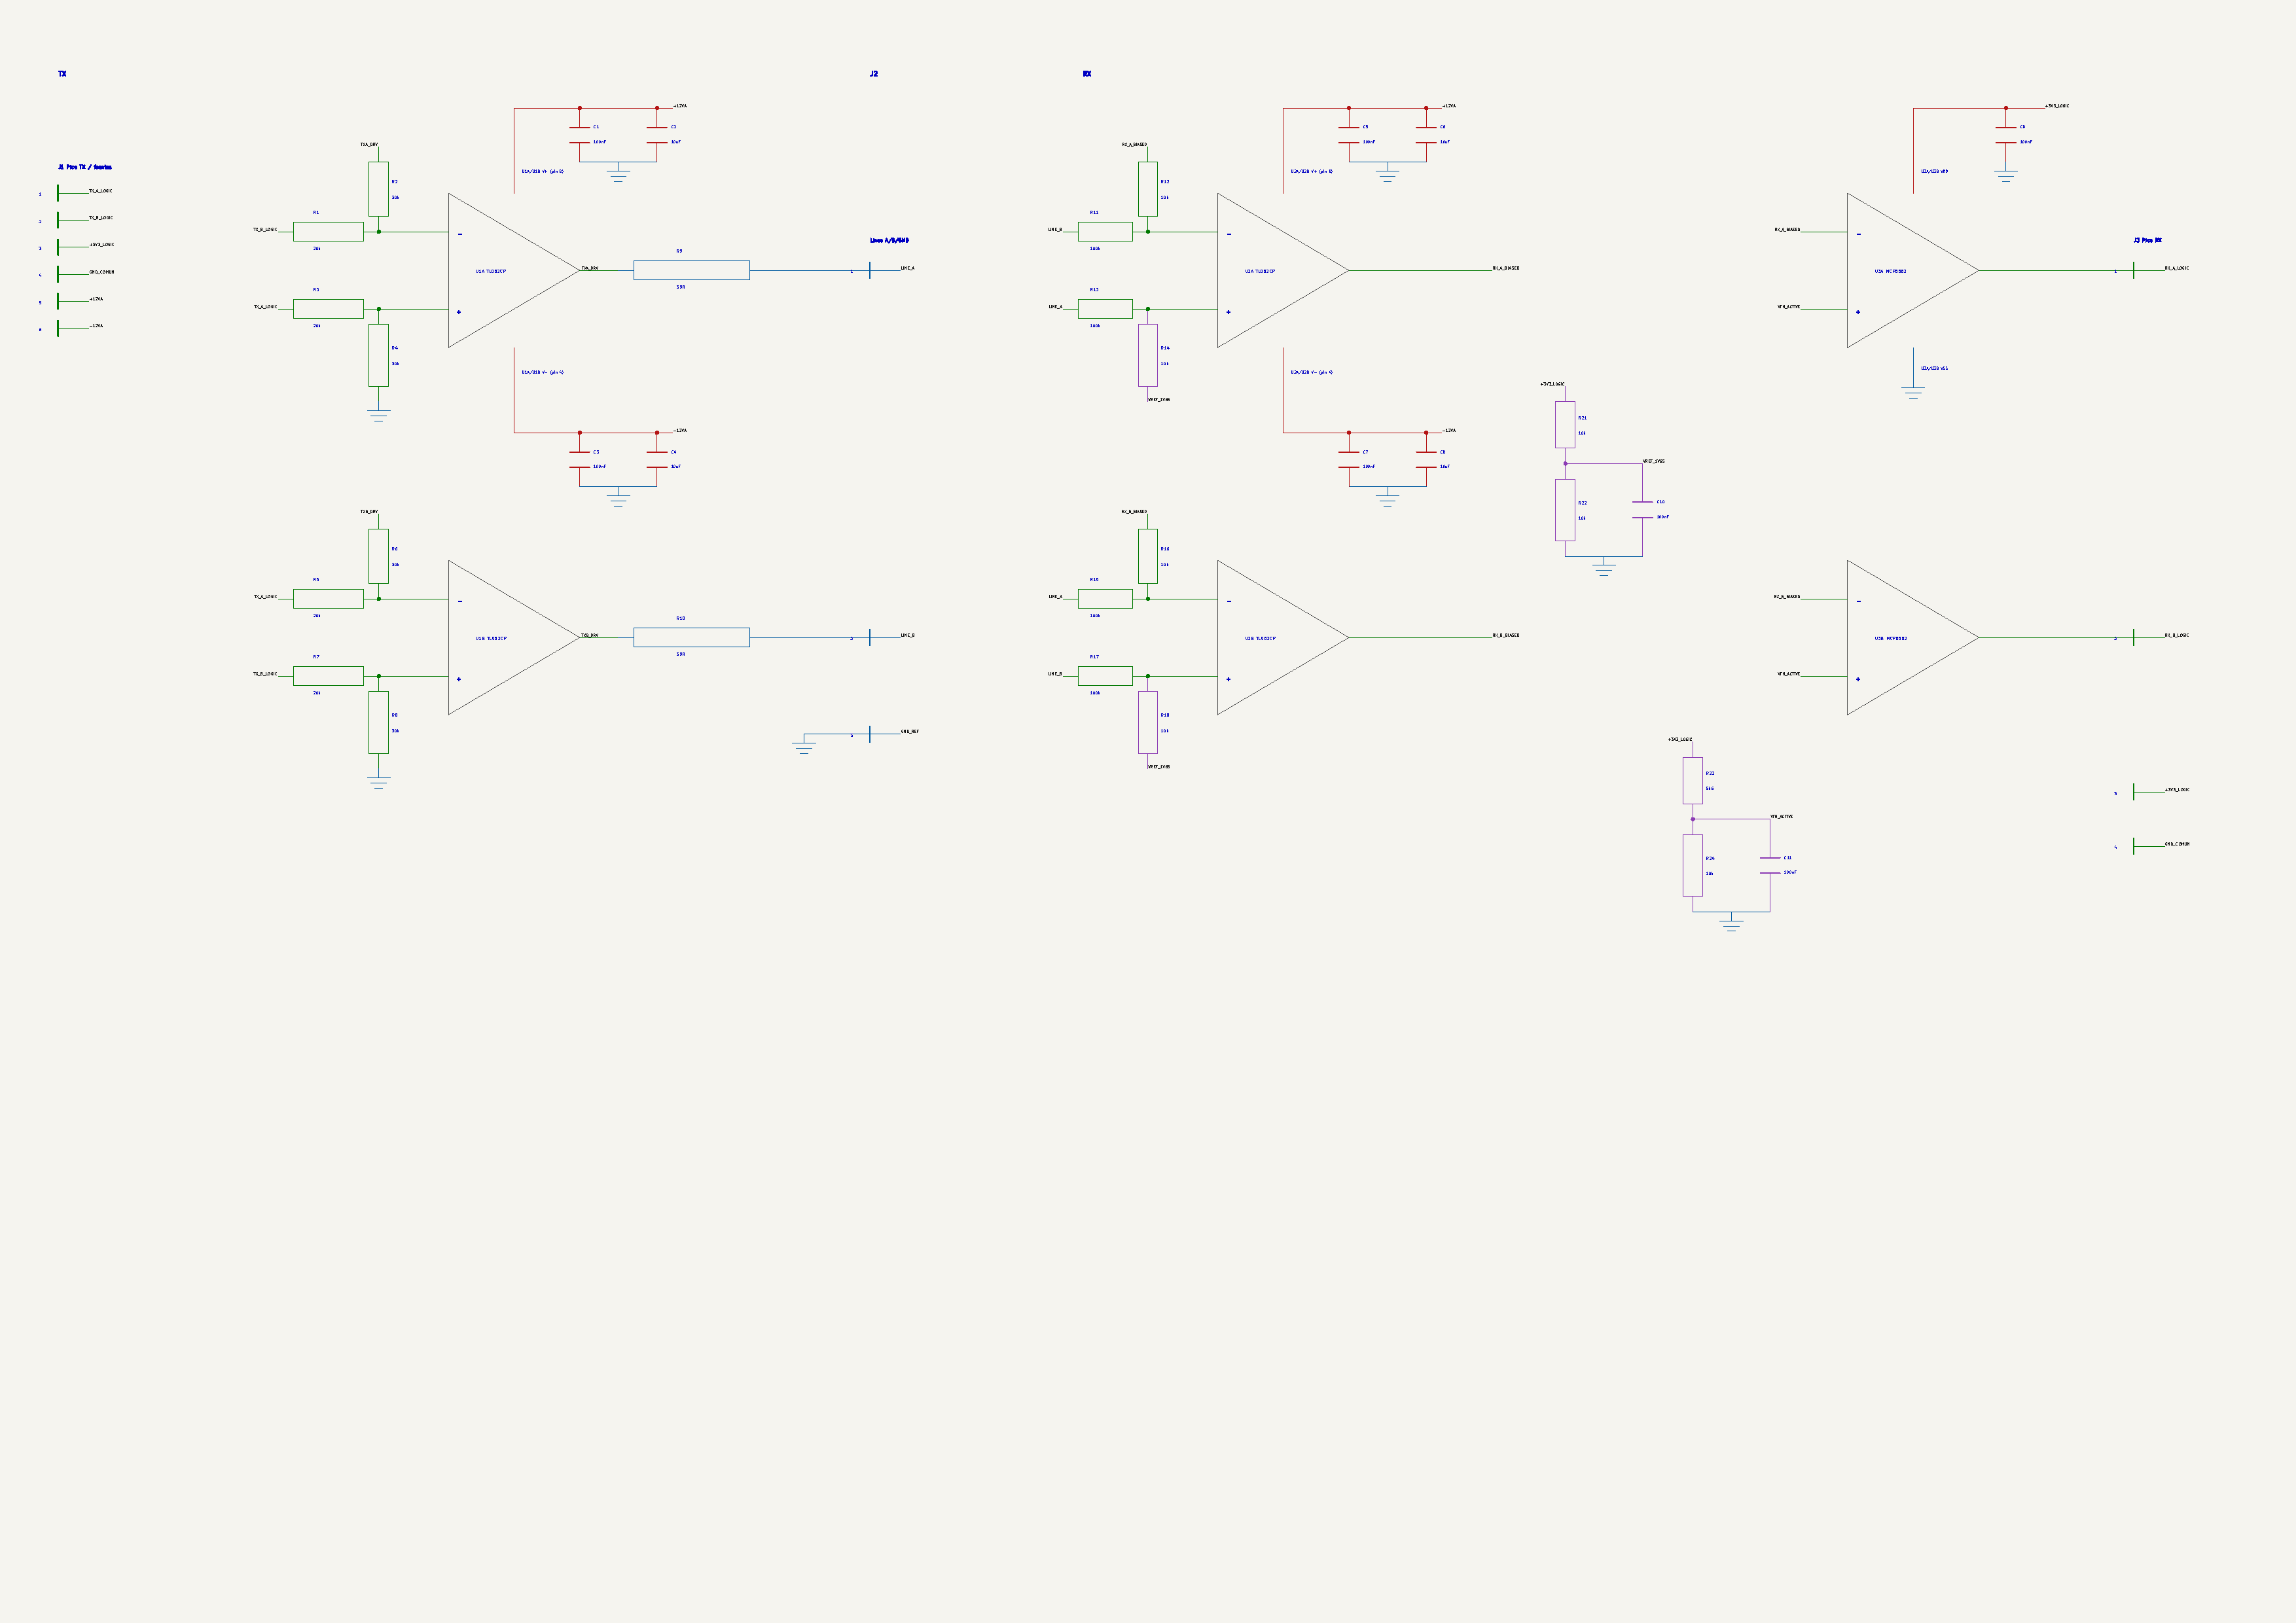
\includegraphics[width=\linewidth,height=0.70\textheight,keepaspectratio,
  trim=20 420 20 15,clip]
  {exports/frontend_arinc429_tl082_circuit.pdf}
\end{center}
\end{landscape}

\section{Fuentes técnicas}

\begin{enumerate}
  \item Texas Instruments, \emph{TL08xx JFET-Input Operational Amplifiers},
  documento SLOS081I, revisión mayo de 2015. Archivo de trabajo:
  \component{TL082CP.pdf}. Información de producto vigente:
  \url{https://www.ti.com/product/TL082}.

  \item AIM GmbH, \emph{ARINC 429 Specification Tutorial}, versión 2.2, julio
  de 2019. Archivo de trabajo:
  \component{aim-tutorial-oview429-190712-u.pdf}.

  \item Microchip Technology, \emph{MCP6561/1R/1U/2/4 -- 1.8V Low-Power
  Push-Pull Output Comparator}, DS20002139E, 2020:
  \url{https://www.microchip.com/en-us/product/MCP6562}.

  \item Proyecto PAMPA, esquemático KiCad
  \component{frontend\_arinc429\_tl082\_circuit.kicad\_sch}, revisión vigente.
\end{enumerate}

\end{document}
